\documentclass[twocolumn]{article}
\usepackage{amsmath, amssymb, amsthm, bm}
\usepackage{graphicx, epsdice, xcolor, listings}
\usepackage[top=1.35in, bottom=1.35in, left=1.35in, right=1.35in]{geometry}

\usepackage{etoolbox}
\patchcmd{\thebibliography}{\section*{\refname}}{}{}{}

\newcommand{\EE}{\mathbb{E}}
\newcommand{\PP}{\mathbb{P}}
\newcommand{\RR}{\mathbb{R}}
%
\newcommand{\Dd}{\mathcal{D}}
\newcommand{\Ee}{\mathcal{E}}
\newcommand{\Gg}{\mathcal{G}}
\newcommand{\Hh}{\mathcal{H}}
\newcommand{\Ii}{\mathcal{I}}
\newcommand{\Kk}{\mathcal{K}}
\newcommand{\Ll}{\mathcal{L}}
\newcommand{\Ss}{\mathcal{S}}
\newcommand{\Tt}{\mathcal{T}}
\newcommand{\Uu}{\mathcal{U}}
\newcommand{\Vv}{\mathcal{V}}
\newcommand{\Xx}{\mathcal{X}}
\newcommand{\Yy}{\mathcal{Y}}

\newcommand{\Ein} {\text{trn}_{\Ss}} %{\Ee_{\text{in},\Uu}}
\newcommand{\Einb} {\text{trn}_{\check\Ss}} %{\Ee_{\text{in},\Uu}}
\newcommand{\Einc} {\text{trn}_{\Ss\sqcup \check\Ss}} %{\Ee_{\text{in},\Uu}}
\newcommand{\Egap}{\text{gap}_{\Ss}}
\newcommand{\Eout}{\text{tst}} %{\Ee_{\text{out}}}

\newtheorem{qst}{Question}
\newtheorem{thm}{Theorem}
\newtheorem{lem}{Lemma}
\theoremstyle{definition}
\newtheorem{dfn}{Definition}
\newtheorem{clm}{Claim}

\begin{document}

    \twocolumn[
        \begin{@twocolumnfalse}
            \begin{flushleft}  \Huge  \emph{What is...} \vspace{0.1cm}\\\hrule \end{flushleft}
            \begin{flushright} \Huge  the Vapnik-Chervonenkis Dimension?     \end{flushright}
            \begin{flushright} \Large Samuel C.\ Tenka      \end{flushright}
        \end{@twocolumnfalse}
    ]

    \subsection*{Wetzel's Cake Problem}

        Mathematicians and bakers alike know the sequence $1, 2, 4, 8, 16, \cdots$
        by heart.  It continues, of course, with $31$, for its $n$th element $p(n)$
        counts the pieces obtained from a disk-shaped cake by cutting along all
        ${n\choose 2}$ lines determined by $n$ generic points on the
        cake's boundary.

        \begin{figure}[h!]
            \centering
            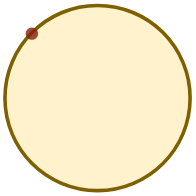
\includegraphics[height=2.3cm]{cake-1}
            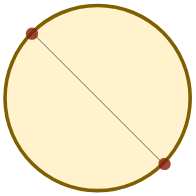
\includegraphics[height=2.3cm]{cake-2}
            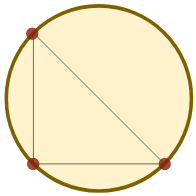
\includegraphics[height=2.3cm]{cake-3}
            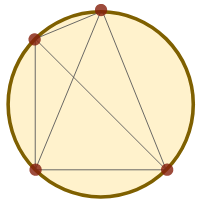
\includegraphics[height=2.3cm]{cake-4}
            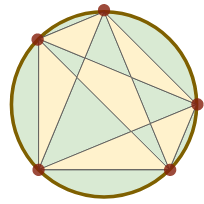
\includegraphics[height=2.3cm]{cake-5-col}
            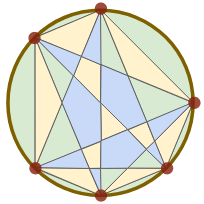
\includegraphics[height=2.3cm]{cake-6-col}
            \caption{\emph{
                Cakes for $n=1, \cdots, 6$.
                The $n=4$ cake (bottom left) has $p(4)=8$ pieces.  We
                color some pieces to make them easier to see and
                to count.  $p(6)$ is clearly odd: the
                pieces besides the central yellow triangle group into sets
                of six.
            }}
        \end{figure}

        Rather than growing exponentially, $p(n)$ is a polynomial \cite{wetzel}.  We may
        compute $p(n)$ by regarding each sliced cake as a planar graph,
        observing that each interior point is determined by two cuts and hence
        by one of ${n\choose 4}$ many sets of $4$ boundary points, and then
        applying Euler's polyhedron formula.  One finds that $p(n)$ is ${n-1
        \choose 0}+\cdots+{n-1\choose 4}$, which explains why $p(n)$ initially
        coincides with $2^{n-1}$.

        This example, like many others in mathematics and in science, serves as
        a warning and a mystery: patterns do not always generalize.  But then
        --- \emph{how is learning from finite data possible at all}? 

        \subsection*{Learning and Generalization}

        We thus wonder: if from a collection $\Hh$ of possible patterns we find
        some $f\in \Hh$ that matches $N$ observed data points, \emph{when
        should we expect that $f$ matches unseen data}?  This question
        motivates machine learning theory and guides machine learning practice.
        
        We may frame the problem in the setting of image classification,
        where $\Xx$ is a space of images, $\{\pm 1\} = \{\text{Cow}, \text{Dog}\}$ is
        a set of (for simplicity, two) labels, and we seek a classifier
        $f: \Xx\to\{\pm 1\}$ that accords with nature.
        More precisely, we posit a probability distribution $\Dd$ over the space
        $\{\pm 1\}\times\Xx$ of labeled images and we let $\Hh \subseteq \{\pm
        1\}^\Xx$ be a set of (measurable) functions.  If $\Ss \sim \Dd^N$ denotes a
        sequence of $N$ observations drawn independently from $\Dd$, the
        \textbf{in-sample error} of $f\in \Hh$ is 
        $$
            \Ein(f) = \PP_{(x,y)\sim \Ss}[f(x)\neq y] 
        $$
        and the \textbf{out-of-sample error} is 
        $$
            \Eout(f) = \PP_{(x,y)\sim \Dd}[f(x)\neq y] 
        $$
        A \textbf{learning rule} $\Ll: (\{\pm 1\}\times\Xx)^N \to \Hh$ maps
        $\Ss$s to $f$s.
        %
        Often, $\Ll$ is induced by an approximate minimization of the in-sample
        error.  However, as the goal of machine learning is typically to 
        achieve out-of-sample error, 
        %
        we wonder when a small in-sample error implies a
        small out-of-sample error, that is, when we may bound the
        \textbf{generalization gap} 
        $$
            \Egap(\Ll) = \Eout(\Ll(\Ss)) - \Ein(\Ll(\Ss)) 
        $$
        In degenerate cases where $\Ll(\Ss)$ and $\Ss$ are independent,
        $\Ein(\Ll(\Ss))$ is an unbiased estimator for $\Eout(\Ll(\Ss))$; by
        laws of large numbers, $\Egap$ is small for large $N$.  The key question
        is:
        \emph{can we control the gap when $\Ll(\Ss)$ depends on $\Ss$}?
        %

        The answer is affirmative when $\Hh$ is ``finite-dimensional'' for a
        certain notion of dimension.  The two ingredients in the story are
        \emph{concentration} and \emph{symmetrization}.

    \subsection*{Concentration}

        \begin{lem}[Chernoff]
            The fraction of heads among $N$ i.i.d.\ flips of a biased coin
            exceeds its mean $p$ by more than $g$ with probability at most 
            $\exp(-Ng^2)$, whenever $p, g, p+g \in[0,1]$.
        \end{lem}

        \begin{proof}
                \begin{figure}[h!]
                    \centering
                    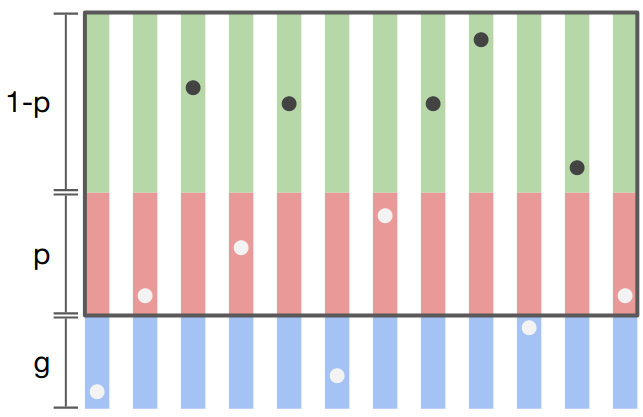
\includegraphics[height=4cm]{chernoff}
                    \caption{\emph{
                        We uniformly randomly sample points on $N$
                        sticks, each with three parts: \textbf{green}
                        with length $1-p$, \textbf{red} with length $p$, and
                        \textbf{blue} with length $g$.  We call non-blue points
                        \textbf{boxed} and non-green points \textbf{hollow}.
                    }}
                    \label{fig:chernoff}
                \end{figure}

                Let our coin flips arise from sampling points on sticks
                (Figure \ref{fig:chernoff}), where green is tails and red
                is heads.
                %
                We'll show that probably less than $(p+g)N = p^\prime N$ flips
                are heads.  That is --- given that all points are
                \textbf{boxed} --- probably less than $p^\prime N$ points are
                red. 
                %
                For any $M\geq p^\prime N$:
                {\small 
                \begin{align*}
                        & ~ \PP[\text{$M$ are red $\mid$ all are boxed}] \\
                      = & ~ \PP[\text{$M$ red and all are boxed}] ~/~ \PP[\text{all are boxed}]  \\
                      = & ~ \PP[\text{$M$ hollow}] \cdot
                            \frac{\PP[\text{all hollows are red $\mid$ $M$ hollow}]}{\PP[\text{all are boxed}]} \\
                      = & ~ \PP[\text{$M$ hollow}] \cdot (1 - g/p^\prime)^{M} ~/~ (1+g)^{-N} 
                \end{align*}
                }
                Since the above holds for all $M\geq p^\prime N$, the chance of too many
                heads is:
                \begin{align*}
                    &~\PP[\text{at least $p^\prime N$ are red $\mid$ all are boxed}] \\
                    \leq
                    &~(1 - g/p^\prime)^{p^\prime N} \cdot (1 + g/p^\prime)^{p^\prime N}
                \end{align*}
                We finish using difference of squares and the convexity of
                $\exp$.
        \end{proof}

        The Chernoff bound gives us the control over tails we'd expect from the
        Central Limit Theorem, but for finite instead of asymptotically large
        $N$.  In particular, when we learn from much but finite data, the
        in-sample error will concentrate near the out-of-sample error.

        For any $f\in \Hh$, $\Ein(f)$ is the average of $N$ independent 
        Bernoullis of mean $\Eout(f)$.  So for $\Hh$ finite and $N$
        large, the gap is probably small:
        \begin{align*}
            &~\PP_{\Ss\sim \Dd^N}[\Egap(\Ll) \geq g] \\
            \leq 
            &~\sum_{f\in \Hh} \PP_{\Ss\sim \Dd^N}[\Eout(f) \geq \Ein(f) + g] \\
            \leq
            &~|\Hh| \cdot \exp(-Ng^2)
        \end{align*}

        For example, if $\Hh$ is parameterized by $P$ numbers, each represented on
        a computer by $32$ bits, then $|\Hh|\leq 2^P$ and, with probability
        $1-\delta$, the gap is no more than
        $$
            \sqrt{(\log(1/\delta) + 32 P)/N}
        $$
        But shouldn't $32$ bits or $64$ bits or infinitely many bits yield similar
        behavior?  Intuitively, the $\Hh$s used in practice --- for instance,
        linear models or neural networks --- depend smoothly on their parameters;
        tiny changes in the parameters yield practically the same classifier, so
        $\Hh$'s cardinality is not an apt measure of its size.  As we will see, the
        V-C dimension measures $\Hh$ more subtly.

    \subsection*{Symmetrization}

        Though $\Hh$ may be infinite, the restriction $\Hh_S = \{f|_S : f
        \in \Hh\}$ is finite for finite $S$.  If we train and test on 
        finitely many points total, we may treat $\Hh$ as finite.  Thus, let
        us estimate $\Eout(f)$, which is an expectation over all of $\Dd$, by
        $\Einb(f)$, an expectation over fresh samples $\check\Ss\sim \Dd^N$
        independent from the samples $\Ss$ on which we learn.

        To show that $\Ein + g \leq \Eout$ when evaluated at $\Ll(\Ss)$, we
        simply show that $\Ein + g/2 \leq \Einb$ and that $\Eout \leq \Einb +
        g/2$.  The former usually holds, since $|\Hh_{\Ss\sqcup\check\Ss}|$ is
        finite; the latter usually holds, since $\Ss$ and $\check\Ss$ are
        independent.  Quantifying with Chernoff, we find that $\Egap(\Ll)$
        exceeds $g$ with chance at most
        \begin{align*}
            \max_{|\Ss|=|\check\Ss|=N}
            |\Hh_{\Ss\sqcup\check\Ss}| ~\cdot~ 2 \cdot \exp(-Ng^2/16)
        \end{align*}
        Thus, to show that the gap is usually small, we need only bound
        $H(n) = \max_{|S|=n} |\Hh_S|$.

        \begin{clm}[Sauer]
        Clearly, $H(n) \leq 2^n$.  In fact, this bound is never somewhat tight:
        depending on $\Hh$, it either is an equality or very loose!
        \end{clm}

        \begin{proof}
        Indeed, consider $\Hh_S$ for $|S|=n$.  Ordering $S$,
        let us write each $f\in \Hh_S$ as a string of $+$s
        and $-$s.  We will count these strings by translating them from the
        alphabet $\{+,-\}$ to the alphabet $\{\blacksquare,\square\}$.
        %
        Intuitively, $\blacksquare$ represents ``surprisingly $+$''.
        More precisely, working from left to right, whenever two
        (partially translated) strings differ \textbf{only} in their
        leftmost untranslated coordinate we overwrite the $+$ version's
        $+$ by $\blacksquare$.  Otherwise, we overwrite by $\square$.

        \definecolor{moor}{rgb}{0.85,0.1 ,0.1 }
        \definecolor{moog}{rgb}{0.1 ,0.75,0.1 }
        \definecolor{moob}{rgb}{0.2 ,0.4 ,1.0 }
        \newcommand{\rR}[1]{{\color{moor}#1}}
        \newcommand{\gG}[1]{{\color{moog}#1}}
        \newcommand{\bB}[1]{{\color{moob}#1}}
        \newcommand{\E}{\texttt{$\square$}}
        \newcommand{\D}{\texttt{$\blacksquare$}}
        \newcommand{\A}{\texttt{$\bm{+}$}}
        \newcommand{\M}{\texttt{$\bm{-}$}}
        \begin{figure}[h]
            \centering
            \resizebox{\columnwidth}{!}{
                \begin{tabular}{ccccccccc}
                       \A \M \M \M  &       &  \E \gG\M \M \M  &       &  \E \E \rR\M \M  &       &  \E \E \E \rR\M  &       &  \E \E \E \E  \\
                       \M \A \M \M  &       &  \E \gG\A \M \M  &       &  \E \D    \M \M  &       &  \E \D \E \bB\M  &       &  \E \D \E \E  \\
                       \M \M \A \M  &       &  \E    \M \A \M  &       &  \E \E \rR\A \M  &       &  \E \E \D \gG\M  &       &  \E \E \D \E  \\
                       \M \M \M \A  & $\to$ &  \E    \M \M \A  & $\to$ &  \E \E \gG\M \A  & $\to$ &  \E \E \E \rR\A  & $\to$ &  \E \E \E \D  \\
                       \M \M \A \A  &       &  \E \bB\M \A \A  &       &  \E \E \gG\A \A  &       &  \E \E \D \gG\A  &       &  \E \E \D \D  \\
                    \rR\M \A \A \A  &       &  \E \bB\A \A \A  &       &  \E \D    \A \A  &       &  \E \D \E \bB\A  &       &  \E \D \E \D  \\
                    \rR\A \A \A \A  &       &  \D    \A \A \A  &       &  \D \E    \A \A  &       &  \D \E \E    \A  &       &  \D \E \E \E
                \end{tabular}
            }
            \caption{
                Translating elements of $H_S$ (left) to strings of choice
                points (right).  Each row corresponds to one of $7$ classifiers
                and each column corresponds to one of $4$ data points.
                %
                We color pairs of strings that differ in-and-only-in their
                leftmost untranslated coordinate.
            }
            \label{fig:sauer}
        \end{figure}

        Each step of translation keeps distinct strings distinct.
        %
        Moreover, whenever some $k$ indices $T\subseteq S$ of a translated string
        are $\blacksquare$s, $|\Hh_T| = 2^k$.  This is because $\blacksquare$s mark
        choice points where the classifiers attain both $+$ and $-$.
        %
        Now, \textbf{either} $H(n)=2^n$ for all $n$, \textbf{or} there is a greatest
        $k$ for which $H(k) = 2^k$.
        In the latter case, no translated string may have more than $k$
        $\blacksquare$s.  Thus $\Hh_S$ contains no more strings than
        there are subsets in $S$ of size $\leq k$.  Therefore,
        $$
            H(n)
            \leq 
            {n\choose 0} + {n\choose 1} + \cdots + {n\choose k}
            \leq 
            (n+2)^{k}
        $$
        As with Cake, what might have grown like $2^n$ grows only
        polynomially.
    \end{proof}

    Intuitively, the exponent $k$ is a dimension: 
    \begin{dfn}
        The \textbf{Vapnik-Chervonenkis dimension} $\text{dim}(\Hh)$ of
        $\Hh \subseteq \{\pm 1\}^\Xx$ is the supremal $k$ for which $H(k) =
        \max_{|S|=k} |\Hh_S| = 2^k$.  
    \end{dfn}
    We conclude that $\Egap(\Ll)$ exceeds $g$ with chance at most
    \begin{align}
        \label{eqn:vc}
       (2N+2)^{\text{dim}(\Hh)} \cdot \exp(-Ng^2/16) \cdot 2
    \end{align}
    For sufficiently large but finite $N$, the gap is small, so
    generalizing from data is possible.

    \subsection*{Statistical Learning Theory}

        The following theorem, whose ``only if'' direction we have sketched above,
        summarizes the V-C dimension's importance to learning theory:
        \begin{thm}[Vapnik and Chervonenkis, 1971]
            The V-C dimension of $\Hh$ is finite if and only if for all data
            distributions $\Dd$, learning rules $\Ll$, and gap bounds $g>0$, the
            chance that $\Egap(\Ll)$ exceeds $g$ tends to $0$ as $N=|\Ss|$ grows.  
        \end{thm}

        For example, if $\Xx$ is a $d$-dimensional real vector space, $\Xx^*$ is
        its dual, and
        $$
            \Hh = \{
                \text{sign} \circ \theta
                :
                \theta \in \Xx^*
            \}
        $$
        is the set of ``linear classifiers'', then $\Hh$'s V-C dimension 
        is at most $d$, because any $d+1$ points $x_0, x_1,\cdots x_d \in
        \Xx$ must participate in a linear relation
        $
            \sum_{i\in I} c_i x_i
            =
            \sum_{j\in J} c_j x_j
        $
        for some $I,J$ disjoint and each $c$ positive, so no $f\in \Hh$
        classifies each $x_i$ as positive and each $x_j$ as negative.  By bound
        \ref{eqn:vc}, a learned linear classifier will generalize when $N \gg d
        \log(N)$.

        %

        Beyond the V-C theorem, \textbf{statistical
        learning theory} abounds with variations on
        the theme that $\Egap \leq \sqrt{\log(|\Hh|/\delta)/N}$.

        For instance, viewing $\log(|\Hh|)$ as the maximum entropy of $\Ll(\Ss)
        \in \Hh$, one may seek tighter bounds given information-theoretic
        data.  Recent progress \cite{abbe} uses the mutual
        information between the random variables $\Ss$ and $\Ll(\Ss)$.

        In another direction, absent control over $\Dd$, one may seek to
        estimate properties of $\Dd$ from $\Ss$.  For instance, \emph{margin
        bounds} detect when $\Dd$'s two classes are geometrically
        well-separated and hence generalization is probable \cite{mohri}.

        Other work specifically analyzes deep neural networks (nets).  The V-C
        bound is empirically very loose for nets.  Indeed, though nets seem to
        have nearly exponential $H(n)$s for $n$ comparable to modern dataset
        sizes \cite{bengio}, they achieve state-of-the-art out-of-sample errors
        on a variety of real-world tasks \cite{hinton}.  A large $H(n)$ means
        that nets are flexible enough to fit arbitrary data.  This flexibility
        allows nets to model complex patterns yet --- in a phenomenon invisible
        to V-C theory --- seems not to hinder generalization.
        %
        Thus, the mystery of modern machine learning: with deep neural
        networks, may we continually halve our cake --- and eat it, too?

    \subsection*{References}
        The use of three-segment sticks and $\{\blacksquare,
        \square\}$-encoding to present the V-C bound is, to the author's
        knowledge, new.  That said, the constant factors throughout this note
        are suboptimal.  The textbook \cite{mohri} surveys learning theory.

        \footnotesize
        \begin{thebibliography}{9}

            \bibitem{vc}
            \textbf{V.\ N.\ Vapnik, A.\ Y.\ Chervonenkis}.
            On uniform convergence of the frequencies of events to their probabilities.
            \textit{Theory of Probability and its Applications}, 1971.

            \bibitem{wetzel}
            \textbf{J.\ E.\ Wetzel}.
            On the Division of the Plane by Lines.
            \textit{The American Mathematical Monthly}, October 1978.

            \bibitem{hinton}
            \textbf{Y.\ LeCun, Y.\ Bengio, G.\ Hinton}.
            Deep Learning.
            \textit{Nature}, 2015.

            \bibitem{bengio}
            \textbf{C.\ Zhang, S.\ Bengio, M.\ Hardt, B.\ Recht, O\. Vinyals}.
            Understanding Deep Learning Requires Rethinking Generalization.
            \textit{International Conference on Learning Representations}, 2017.

            \bibitem{mohri}
            \textbf{M.\ Mohri, A.\ Rostamizadeh, A.\ Talwalkar}.
            Foundations of Machine Learning.
            \textit{MIT Press}, 2018.

            \bibitem{abbe}
            \textbf{A.\ R.\ Asadi, E.\ Abbe, S.\ Verd\'u}.
            Chaining Mutual Information and Tightening Generalization Bounds.
            \textit{Neural Information Processing Systems}, 2018.

        \end{thebibliography}

\end{document}


